\documentclass[12pt]{article}

%packages
%\usepackage{latexsym}
\usepackage{graphicx}
\usepackage{wrapfig}
\usepackage{color}
\usepackage{amsmath}
\usepackage{dsfont}
\usepackage{placeins}
\usepackage{amssymb}
\usepackage{skull}
\usepackage{enumerate}
\usepackage{soul}
\usepackage{alphalph}
\usepackage{hyperref}
\usepackage{enumerate}
\usepackage{listings}
\usepackage{multicol}
%\usepackage{fancyhdr}

%\fancyhf{} % clear all header and footers
%\renewcommand{\headrulewidth}{0pt} % remove the header rule
%\fancyfoot[LE, LO]{\thepage}


%\usepackage{pstricks,pst-node,pst-tree}

%\usepackage{algpseudocode}
%\usepackage{amsthm}
%\usepackage{hyperref}
%\usepackage{mathrsfs}
%\usepackage{amsfonts}
%\usepackage{bbding}
%\usepackage{listings}
%\usepackage{appendix}
\usepackage[margin=1in]{geometry}
%\geometry{papersize={8.5in,11in},total={6.5in,9in}}
%\usepackage{cancel}
%\usepackage{algorithmic, algorithm}

\definecolor{dkgreen}{rgb}{0,0.6,0}
\definecolor{gray}{rgb}{0.5,0.5,0.5}
\definecolor{mauve}{rgb}{0.58,0,0.82}
\lstset{ %
  language=R,                     % the language of the code
  basicstyle=\footnotesize,       % the size of the fonts that are used for the code
  numbers=left,                   % where to put the line-numbers
  numberstyle=\tiny\color{gray},  % the style that is used for the line-numbers
  stepnumber=1,                   % the step between two line-numbers. If it's 1, each line
                                  % will be numbered
  numbersep=5pt,                  % how far the line-numbers are from the code
  backgroundcolor=\color{white},  % choose the background color. You must add \usepackage{color}
  showspaces=false,               % show spaces adding particular underscores
  showstringspaces=false,         % underline spaces within strings
  showtabs=false,                 % show tabs within strings adding particular underscores
  frame=single,                   % adds a frame around the code
  rulecolor=\color{black},        % if not set, the frame-color may be changed on line-breaks within not-black text (e.g. commens (green here))
  tabsize=2,                      % sets default tabsize to 2 spaces
  captionpos=b,                   % sets the caption-position to bottom
  breaklines=true,                % sets automatic line breaking
  breakatwhitespace=false,        % sets if automatic breaks should only happen at whitespace
  title=\lstname,                 % show the filename of files included with \lstinputlisting;
                                  % also try caption instead of title
  keywordstyle=\color{black},      % keyword style
  commentstyle=\color{dkgreen},   % comment style
  stringstyle=\color{mauve},      % string literal style
  escapeinside={\%*}{*)},         % if you want to add a comment within your code
  morekeywords={*,...}            % if you want to add more keywords to the set
}

\newcommand{\qu}[1]{``#1''}
\newcommand{\spc}[1]{\\ \vspace{#1cm}}

\newcounter{probnum}
\setcounter{probnum}{1}

%create definition to allow local margin changes
\def\changemargin#1#2{\list{}{\rightmargin#2\leftmargin#1}\item[]}
\let\endchangemargin=\endlist 

%allow equations to span multiple pages
\allowdisplaybreaks

%define colors and color typesetting conveniences
\definecolor{gray}{rgb}{0.5,0.5,0.5}
\definecolor{black}{rgb}{0,0,0}
\definecolor{white}{rgb}{1,1,1}
\definecolor{blue}{rgb}{0.5,0.5,1}
\newcommand{\inblue}[1]{\color{blue}#1 \color{black}}
\definecolor{green}{rgb}{0.133,0.545,0.133}
\newcommand{\ingreen}[1]{\color{green}#1 \color{black}}
\definecolor{yellow}{rgb}{1,0.549,0}
\newcommand{\inyellow}[1]{\color{yellow}#1 \color{black}}
\definecolor{red}{rgb}{1,0.133,0.133}
\newcommand{\inred}[1]{\color{red}#1 \color{black}}
\definecolor{purple}{rgb}{0.58,0,0.827}
\newcommand{\inpurple}[1]{\color{purple}#1 \color{black}}
\definecolor{gray}{rgb}{0.5,0.5,0.5}
\newcommand{\ingray}[1]{\color{gray}#1 \color{black}}
\definecolor{backgcode}{rgb}{0.97,0.97,0.8}
\definecolor{Brown}{cmyk}{0,0.81,1,0.60}
\definecolor{OliveGreen}{cmyk}{0.64,0,0.95,0.40}
\definecolor{CadetBlue}{cmyk}{0.62,0.57,0.23,0}

%define new math operators
\DeclareMathOperator*{\argmax}{arg\,max~}
\DeclareMathOperator*{\argmin}{arg\,min~}
\DeclareMathOperator*{\argsup}{arg\,sup~}
\DeclareMathOperator*{\arginf}{arg\,inf~}
\DeclareMathOperator*{\convolution}{\text{\Huge{$\ast$}}}
\newcommand{\infconv}[2]{\convolution^\infty_{#1 = 1} #2}
%true functions

%%%% GENERAL SHORTCUTS

\makeatletter
\newalphalph{\alphmult}[mult]{\@alph}{26}
\renewcommand{\labelenumi}{(\alphmult{\value{enumi}})}
\renewcommand{\theenumi}{\AlphAlph{\value{enumi}}}
\makeatother
%shortcuts for pure typesetting conveniences
\newcommand{\bv}[1]{\boldsymbol{#1}}

%shortcuts for compound constants
\newcommand{\BetaDistrConst}{\dfrac{\Gamma(\alpha + \beta)}{\Gamma(\alpha)\Gamma(\beta)}}
\newcommand{\NormDistrConst}{\dfrac{1}{\sqrt{2\pi\sigma^2}}}

%shortcuts for conventional symbols
\newcommand{\tsq}{\tau^2}
\newcommand{\tsqh}{\hat{\tau}^2}
\newcommand{\sigsq}{\sigma^2}
\newcommand{\sigsqsq}{\parens{\sigma^2}^2}
\newcommand{\sigsqovern}{\dfrac{\sigsq}{n}}
\newcommand{\tausq}{\tau^2}
\newcommand{\tausqalpha}{\tau^2_\alpha}
\newcommand{\tausqbeta}{\tau^2_\beta}
\newcommand{\tausqsigma}{\tau^2_\sigma}
\newcommand{\betasq}{\beta^2}
\newcommand{\sigsqvec}{\bv{\sigma}^2}
\newcommand{\sigsqhat}{\hat{\sigma}^2}
\newcommand{\sigsqhatmlebayes}{\sigsqhat_{\text{Bayes, MLE}}}
\newcommand{\sigsqhatmle}[1]{\sigsqhat_{#1, \text{MLE}}}
\newcommand{\bSigma}{\bv{\Sigma}}
\newcommand{\bSigmainv}{\bSigma^{-1}}
\newcommand{\thetavec}{\bv{\theta}}
\newcommand{\thetahat}{\hat{\theta}}
\newcommand{\thetahatmm}{\hat{\theta}^{\mathrm{MM}}}
\newcommand{\thetahathatmm}{\thetahathat^{\mathrm{MM}}}
\newcommand{\thetahathatmle}{\thetahathat^{\mathrm{MLE}}}
\newcommand{\thetahatmle}{\hat{\theta}^{\mathrm{MLE}}}
\newcommand{\thetavechatmle}{\hat{\thetavec}^{\mathrm{MLE}}}
\newcommand{\muhat}{\hat{\mu}}
\newcommand{\musq}{\mu^2}
\newcommand{\muvec}{\bv{\mu}}
\newcommand{\muhatmle}{\muhat_{\text{MLE}}}
\newcommand{\lambdahat}{\hat{\lambda}}
\newcommand{\lambdahatmle}{\lambdahat_{\text{MLE}}}
\newcommand{\thetahatmap}{\hat{\theta}_{\mathrm{MAP}}}
\newcommand{\thetahatmmae}{\hat{\theta}_{\mathrm{MMAE}}}
\newcommand{\thetahatmmse}{\hat{\theta}_{\mathrm{MMSE}}}
\newcommand{\etavec}{\bv{\eta}}
\newcommand{\alphavec}{\bv{\alpha}}
\newcommand{\minimaxdec}{\delta^*_{\mathrm{mm}}}
\newcommand{\ybar}{\bar{y}}
\newcommand{\xbar}{\bar{x}}
\newcommand{\Xbar}{\bar{X}}
\newcommand{\iid}{~{\buildrel iid \over \sim}~}
\newcommand{\inddist}{~{\buildrel ind \over \sim}~}
\newcommand{\approxdist}{~{\buildrel \bv{\cdot} \over \sim}~}
\newcommand{\equalsindist}{~{\buildrel d \over =}~}
\newcommand{\loglik}[1]{\ell\parens{#1}}
\newcommand{\thetahatkminone}{\thetahat^{(k-1)}}
\newcommand{\thetahatkplusone}{\thetahat^{(k+1)}}
\newcommand{\thetahatk}{\thetahat^{(k)}}
\newcommand{\half}{\frac{1}{2}}
\newcommand{\third}{\frac{1}{3}}
\newcommand{\twothirds}{\frac{2}{3}}
\newcommand{\fourth}{\frac{1}{4}}
\newcommand{\fifth}{\frac{1}{5}}
\newcommand{\sixth}{\frac{1}{6}}

%shortcuts for vector and matrix notation
\newcommand{\A}{\bv{A}}
\newcommand{\At}{\A^T}
\newcommand{\Ainv}{\inverse{\A}}
\newcommand{\B}{\bv{B}}
\renewcommand{\b}{\bv{b}}
\renewcommand{\H}{\bv{H}}
\newcommand{\K}{\bv{K}}
\newcommand{\Kt}{\K^T}
\newcommand{\Kinv}{\inverse{K}}
\newcommand{\Kinvt}{(\Kinv)^T}
\newcommand{\M}{\bv{M}}
\newcommand{\Bt}{\B^T}
\newcommand{\Q}{\bv{Q}}
\newcommand{\Qt}{\Q^T}
\newcommand{\R}{\bv{R}}
\newcommand{\Rt}{\R^T}
\newcommand{\Z}{\bv{Z}}
\newcommand{\X}{\bv{X}}
\newcommand{\Xsub}{\X_{\text{(sub)}}}
\newcommand{\Xsubadj}{\X_{\text{(sub,adj)}}}
\newcommand{\I}{\bv{I}}
\newcommand{\Y}{\bv{Y}}
\newcommand{\sigsqI}{\sigsq\I}
\renewcommand{\P}{\bv{P}}
\newcommand{\Psub}{\P_{\text{(sub)}}}
\newcommand{\Pt}{\P^T}
\newcommand{\Pii}{P_{ii}}
\newcommand{\Pij}{P_{ij}}
\newcommand{\IminP}{(\I-\P)}
\newcommand{\Xt}{\bv{X}^T}
\newcommand{\XtX}{\Xt\X}
\newcommand{\XtXinv}{\parens{\Xt\X}^{-1}}
\newcommand{\XtXinvXt}{\XtXinv\Xt}
\newcommand{\XXtXinvXt}{\X\XtXinvXt}
\newcommand{\x}{\bv{x}}
\newcommand{\w}{\bv{w}}
\newcommand{\q}{\bv{q}}
\newcommand{\zerovec}{\bv{0}}
\newcommand{\onevec}{\bv{1}}
\newcommand{\oneton}{1, \ldots, n}
\newcommand{\yoneton}{y_1, \ldots, y_n}
\newcommand{\yonetonorder}{y_{(1)}, \ldots, y_{(n)}}
\newcommand{\Yoneton}{Y_1, \ldots, Y_n}
\newcommand{\iinoneton}{i \in \braces{\oneton}}
\newcommand{\onetom}{1, \ldots, m}
\newcommand{\jinonetom}{j \in \braces{\onetom}}
\newcommand{\xoneton}{x_1, \ldots, x_n}
\newcommand{\Xoneton}{X_1, \ldots, X_n}
\newcommand{\xt}{\x^T}
\newcommand{\y}{\bv{y}}
\newcommand{\yt}{\y^T}
\renewcommand{\c}{\bv{c}}
\newcommand{\ct}{\c^T}
\newcommand{\tstar}{\bv{t}^*}
\renewcommand{\u}{\bv{u}}
\renewcommand{\v}{\bv{v}}
\renewcommand{\a}{\bv{a}}
\newcommand{\s}{\bv{s}}
\newcommand{\yadj}{\y_{\text{(adj)}}}
\newcommand{\xjadj}{\x_{j\text{(adj)}}}
\newcommand{\xjadjM}{\x_{j \perp M}}
\newcommand{\yhat}{\hat{\y}}
\newcommand{\yhatsub}{\yhat_{\text{(sub)}}}
\newcommand{\yhatstar}{\yhat^*}
\newcommand{\yhatstarnew}{\yhatstar_{\text{new}}}
\newcommand{\z}{\bv{z}}
\newcommand{\zt}{\z^T}
\newcommand{\bb}{\bv{b}}
\newcommand{\bbt}{\bb^T}
\newcommand{\bbeta}{\bv{\beta}}
\newcommand{\beps}{\bv{\epsilon}}
\newcommand{\bepst}{\beps^T}
\newcommand{\e}{\bv{e}}
\newcommand{\Mofy}{\M(\y)}
\newcommand{\KofAlpha}{K(\alpha)}
\newcommand{\ellset}{\mathcal{L}}
\newcommand{\oneminalph}{1-\alpha}
\newcommand{\SSE}{\text{SSE}}
\newcommand{\SSEsub}{\text{SSE}_{\text{(sub)}}}
\newcommand{\MSE}{\text{MSE}}
\newcommand{\RMSE}{\text{RMSE}}
\newcommand{\SSR}{\text{SSR}}
\newcommand{\SST}{\text{SST}}
\newcommand{\JSest}{\delta_{\text{JS}}(\x)}
\newcommand{\Bayesest}{\delta_{\text{Bayes}}(\x)}
\newcommand{\EmpBayesest}{\delta_{\text{EmpBayes}}(\x)}
\newcommand{\BLUPest}{\delta_{\text{BLUP}}}
\newcommand{\MLEest}[1]{\hat{#1}_{\text{MLE}}}

%shortcuts for Linear Algebra stuff (i.e. vectors and matrices)
\newcommand{\twovec}[2]{\bracks{\begin{array}{c} #1 \\ #2 \end{array}}}
\newcommand{\threevec}[3]{\bracks{\begin{array}{c} #1 \\ #2 \\ #3 \end{array}}}
\newcommand{\fivevec}[5]{\bracks{\begin{array}{c} #1 \\ #2 \\ #3 \\ #4 \\ #5 \end{array}}}
\newcommand{\twobytwomat}[4]{\bracks{\begin{array}{cc} #1 & #2 \\ #3 & #4 \end{array}}}
\newcommand{\threebytwomat}[6]{\bracks{\begin{array}{cc} #1 & #2 \\ #3 & #4 \\ #5 & #6 \end{array}}}

%shortcuts for conventional compound symbols
\newcommand{\thetainthetas}{\theta \in \Theta}
\newcommand{\reals}{\mathbb{R}}
\newcommand{\complexes}{\mathbb{C}}
\newcommand{\rationals}{\mathbb{Q}}
\newcommand{\integers}{\mathbb{Z}}
\newcommand{\naturals}{\mathbb{N}}
\newcommand{\forallninN}{~~\forall n \in \naturals}
\newcommand{\forallxinN}[1]{~~\forall #1 \in \reals}
\newcommand{\matrixdims}[2]{\in \reals^{\,#1 \times #2}}
\newcommand{\inRn}[1]{\in \reals^{\,#1}}
\newcommand{\mathimplies}{\quad\Rightarrow\quad}
\newcommand{\mathlogicequiv}{\quad\Leftrightarrow\quad}
\newcommand{\eqncomment}[1]{\quad \text{(#1)}}
\newcommand{\limitn}{\lim_{n \rightarrow \infty}}
\newcommand{\limitN}{\lim_{N \rightarrow \infty}}
\newcommand{\limitd}{\lim_{d \rightarrow \infty}}
\newcommand{\limitt}{\lim_{t \rightarrow \infty}}
\newcommand{\limitsupn}{\limsup_{n \rightarrow \infty}~}
\newcommand{\limitinfn}{\liminf_{n \rightarrow \infty}~}
\newcommand{\limitk}{\lim_{k \rightarrow \infty}}
\newcommand{\limsupn}{\limsup_{n \rightarrow \infty}}
\newcommand{\limsupk}{\limsup_{k \rightarrow \infty}}
\newcommand{\floor}[1]{\left\lfloor #1 \right\rfloor}
\newcommand{\ceil}[1]{\left\lceil #1 \right\rceil}

%shortcuts for environments
\newcommand{\beqn}{\vspace{-0.25cm}\begin{eqnarray*}}
\newcommand{\eeqn}{\end{eqnarray*}}
\newcommand{\bneqn}{\vspace{-0.25cm}\begin{eqnarray}}
\newcommand{\eneqn}{\end{eqnarray}}
\newcommand{\benum}{\begin{itemize}}
\newcommand{\eenum}{\end{itemize}}

%shortcuts for mini environments
\newcommand{\parens}[1]{\left(#1\right)}
\newcommand{\squared}[1]{\parens{#1}^2}
\newcommand{\tothepow}[2]{\parens{#1}^{#2}}
\newcommand{\prob}[1]{\mathbb{P}\parens{#1}}
\newcommand{\littleo}[1]{o\parens{#1}}
\newcommand{\bigo}[1]{O\parens{#1}}
\newcommand{\Lp}[1]{\mathbb{L}^{#1}}
\renewcommand{\arcsin}[1]{\text{arcsin}\parens{#1}}
\newcommand{\prodonen}[2]{\bracks{\prod_{#1=1}^n #2}}
\newcommand{\mysum}[4]{\sum_{#1=#2}^{#3} #4}
\newcommand{\sumonen}[2]{\sum_{#1=1}^n #2}
\newcommand{\infsum}[2]{\sum_{#1=1}^\infty #2}
\newcommand{\infprod}[2]{\prod_{#1=1}^\infty #2}
\newcommand{\infunion}[2]{\bigcup_{#1=1}^\infty #2}
\newcommand{\infinter}[2]{\bigcap_{#1=1}^\infty #2}
\newcommand{\infintegral}[2]{\int^\infty_{-\infty} #2 ~\text{d}#1}
\newcommand{\supthetas}[1]{\sup_{\thetainthetas}\braces{#1}}
\newcommand{\bracks}[1]{\left[#1\right]}
\newcommand{\braces}[1]{\left\{#1\right\}}
\newcommand{\angbraces}[1]{\left<#1\right>}
\newcommand{\set}[1]{\left\{#1\right\}}
\newcommand{\abss}[1]{\left|#1\right|}
\newcommand{\norm}[1]{\left|\left|#1\right|\right|}
\newcommand{\normsq}[1]{\norm{#1}^2}
\newcommand{\inverse}[1]{\parens{#1}^{-1}}
\newcommand{\rowof}[2]{\parens{#1}_{#2\cdot}}

%shortcuts for functionals
\newcommand{\realcomp}[1]{\text{Re}\bracks{#1}}
\newcommand{\imagcomp}[1]{\text{Im}\bracks{#1}}
\newcommand{\range}[1]{\text{range}\bracks{#1}}
\newcommand{\colsp}[1]{\text{colsp}\bracks{#1}}
\newcommand{\rowsp}[1]{\text{rowsp}\bracks{#1}}
\newcommand{\tr}[1]{\text{tr}\bracks{#1}}
\newcommand{\rank}[1]{\text{rank}\bracks{#1}}
\newcommand{\proj}[2]{\text{Proj}_{#1}\bracks{#2}}
\newcommand{\projcolspX}[1]{\text{Proj}_{\colsp{\X}}\bracks{#1}}
\newcommand{\median}[1]{\text{median}\bracks{#1}}
\newcommand{\mean}[1]{\text{mean}\bracks{#1}}
\newcommand{\dime}[1]{\text{dim}\bracks{#1}}
\renewcommand{\det}[1]{\text{det}\bracks{#1}}
\newcommand{\expe}[1]{\mathbb{E}\bracks{#1}}
\newcommand{\expeabs}[1]{\expe{\abss{#1}}}
\newcommand{\expesub}[2]{\mathbb{E}_{#1}\bracks{#2}}
\newcommand{\cexpesub}[3]{\mathbb{E}_{#1}\bracks{#2~|~#3}}
\newcommand{\indic}[1]{\mathds{1}_{#1}}
\newcommand{\var}[1]{\mathbb{V}\text{ar}\bracks{#1}}
\newcommand{\mse}[1]{\mathbb{M}\text{SE}\bracks{#1}}
\newcommand{\sd}[1]{\mathbb{S}\text{D}\bracks{#1}}
\newcommand{\support}[1]{\mathbb{S}_{#1}}
\newcommand{\cov}[2]{\mathbb{C}\text{ov}\bracks{#1, #2}}
\newcommand{\corr}[2]{\mathbb{C}\text{orr}\bracks{#1, #2}}
\newcommand{\se}[1]{\text{SE}\bracks{#1}}
\newcommand{\seest}[1]{\hat{\text{SE}}\bracks{#1}}
\newcommand{\bias}[1]{\mathbb{B}\text{ias}\bracks{#1}}
\newcommand{\partialop}[2]{\dfrac{\partial}{\partial #1}\bracks{#2}}
\newcommand{\secpartialop}[2]{\dfrac{\partial^2}{\partial #1^2}\bracks{#2}}
\newcommand{\mixpartialop}[3]{\dfrac{\partial^2}{\partial #1 \partial #2}\bracks{#3}}

%shortcuts for functions
\renewcommand{\exp}[1]{\mathrm{exp}\parens{#1}}
\renewcommand{\cos}[1]{\text{cos}\parens{#1}}
\renewcommand{\sin}[1]{\text{sin}\parens{#1}}
\newcommand{\sign}[1]{\text{sign}\parens{#1}}
\newcommand{\are}[1]{\mathrm{ARE}\parens{#1}}
\newcommand{\natlog}[1]{\ln\parens{#1}}
\newcommand{\oneover}[1]{\frac{1}{#1}}
\newcommand{\overtwo}[1]{\frac{#1}{2}}
\newcommand{\overn}[1]{\frac{#1}{n}}
\newcommand{\oversqrtn}[1]{\frac{#1}{\sqrt{n}}}
\newcommand{\oneoversqrt}[1]{\oneover{\sqrt{#1}}}
\newcommand{\sqd}[1]{\parens{#1}^2}
\newcommand{\loss}[1]{\ell\parens{\theta, #1}}
\newcommand{\losstwo}[2]{\ell\parens{#1, #2}}
\newcommand{\cf}{\phi(t)}

%English language specific shortcuts
\newcommand{\ie}{\textit{i.e.} }
\newcommand{\AKA}{\textit{AKA} }
\renewcommand{\iff}{\textit{iff}}
\newcommand{\eg}{\textit{e.g.} }
\renewcommand{\st}{\textit{s.t.} }
\newcommand{\wrt}{\textit{w.r.t.} }
\newcommand{\mathst}{~~\text{\st}~~}
\newcommand{\mathand}{~~\text{and}~~}
\newcommand{\ala}{\textit{a la} }
\newcommand{\ppp}{posterior predictive p-value}
\newcommand{\dd}{dataset-to-dataset}

%shortcuts for distribution titles
\newcommand{\logistic}[2]{\mathrm{Logistic}\parens{#1,\,#2}}
\newcommand{\bernoulli}[1]{\mathrm{Bernoulli}\parens{#1}}
\newcommand{\betanot}[2]{\mathrm{Beta}\parens{#1,\,#2}}
\newcommand{\stdbetanot}{\betanot{\alpha}{\beta}}
\newcommand{\multnormnot}[3]{\mathcal{N}_{#1}\parens{#2,\,#3}}
\newcommand{\normnot}[2]{\mathcal{N}\parens{#1,\,#2}}
\newcommand{\classicnormnot}{\normnot{\mu}{\sigsq}}
\newcommand{\stdnormnot}{\normnot{0}{1}}
\newcommand{\uniform}[2]{\mathrm{U}\parens{#1,\,#2}}
\newcommand{\stduniform}{\uniform{0}{1}}
\newcommand{\exponential}[1]{\mathrm{Exp}\parens{#1}}
\newcommand{\geometric}[1]{\mathrm{Geometric}\parens{#1}}
\newcommand{\gammadist}[2]{\mathrm{Gamma}\parens{#1, #2}}
\newcommand{\negbin}[2]{\mathrm{NegBin}\parens{#1, #2}}
\newcommand{\poisson}[1]{\mathrm{Poisson}\parens{#1}}
\newcommand{\binomial}[2]{\mathrm{Binomial}\parens{#1,\,#2}}
\newcommand{\erlang}[2]{\mathrm{Erlang}\parens{#1,\,#2}}
\newcommand{\rayleigh}[1]{\mathrm{Rayleigh}\parens{#1}}
\newcommand{\multinomial}[3]{\mathrm{Multinom}_{#1}\parens{#2,\,#3}}
\newcommand{\gammanot}[2]{\mathrm{Gamma}\parens{#1,\,#2}}
\newcommand{\cauchynot}[2]{\text{Cauchy}\parens{#1,\,#2}}
\newcommand{\invchisqnot}[1]{\text{Inv}\chisq{#1}}
\newcommand{\invscaledchisqnot}[2]{\text{ScaledInv}\ncchisq{#1}{#2}}
\newcommand{\invgammanot}[2]{\text{InvGamma}\parens{#1,\,#2}}
\newcommand{\chisq}[1]{\chi^2_{#1}}
\newcommand{\ncchisq}[2]{\chi^2_{#1}\parens{#2}}
\newcommand{\ncF}[3]{F_{#1,#2}\parens{#3}}

%shortcuts for PDF's of common distributions
\newcommand{\logisticpdf}[3]{\oneover{#3}\dfrac{\exp{-\dfrac{#1 - #2}{#3}}}{\parens{1+\exp{-\dfrac{#1 - #2}{#3}}}^2}}
\newcommand{\betapdf}[3]{\dfrac{\Gamma(#2 + #3)}{\Gamma(#2)\Gamma(#3)}#1^{#2-1} (1-#1)^{#3-1}}
\newcommand{\normpdf}[3]{\frac{1}{\sqrt{2\pi#3}}\exp{-\frac{1}{2#3}(#1 - #2)^2}}
\newcommand{\normpdfvarone}[2]{\dfrac{1}{\sqrt{2\pi}}e^{-\half(#1 - #2)^2}}
\newcommand{\chisqpdf}[2]{\dfrac{1}{2^{#2/2}\Gamma(#2/2)}\; {#1}^{#2/2-1} e^{-#1/2}}
\newcommand{\invchisqpdf}[2]{\dfrac{2^{-\overtwo{#1}}}{\Gamma(#2/2)}\,{#1}^{-\overtwo{#2}-1}  e^{-\oneover{2 #1}}}
\newcommand{\uniformdiscrete}[1]{\mathrm{Uniform}\parens{\braces{#1}}}
\newcommand{\exponentialpdf}[2]{#2\exp{-#2#1}}
\newcommand{\poissonpdf}[2]{\dfrac{e^{-#1} #1^{#2}}{#2!}}
\newcommand{\binomialpdf}[3]{\binom{#2}{#1}#3^{#1}(1-#3)^{#2-#1}}
\newcommand{\rayleighpdf}[2]{\dfrac{#1}{#2^2}\exp{-\dfrac{#1^2}{2 #2^2}}}
\newcommand{\gammapdf}[3]{\dfrac{#3^#2}{\Gamma\parens{#2}}#1^{#2-1}\exp{-#3 #1}}
\newcommand{\cauchypdf}[3]{\oneover{\pi} \dfrac{#3}{\parens{#1-#2}^2 + #3^2}}
\newcommand{\Gammaf}[1]{\Gamma\parens{#1}}

%shortcuts for miscellaneous typesetting conveniences
\newcommand{\notesref}[1]{\marginpar{\color{gray}\tt #1\color{black}}}

%%%% DOMAIN-SPECIFIC SHORTCUTS

%Real analysis related shortcuts
\newcommand{\zeroonecl}{\bracks{0,1}}
\newcommand{\forallepsgrzero}{\forall \epsilon > 0~~}
\newcommand{\lessthaneps}{< \epsilon}
\newcommand{\fraccomp}[1]{\text{frac}\bracks{#1}}

%Bayesian related shortcuts
\newcommand{\yrep}{y^{\text{rep}}}
\newcommand{\yrepisq}{(\yrep_i)^2}
\newcommand{\yrepvec}{\bv{y}^{\text{rep}}}


%Probability shortcuts
\newcommand{\SigField}{\mathcal{F}}
\newcommand{\ProbMap}{\mathcal{P}}
\newcommand{\probtrinity}{\parens{\Omega, \SigField, \ProbMap}}
\newcommand{\convp}{~{\buildrel p \over \rightarrow}~}
\newcommand{\convLp}[1]{~{\buildrel \Lp{#1} \over \rightarrow}~}
\newcommand{\nconvp}{~{\buildrel p \over \nrightarrow}~}
\newcommand{\convae}{~{\buildrel a.e. \over \longrightarrow}~}
\newcommand{\convau}{~{\buildrel a.u. \over \longrightarrow}~}
\newcommand{\nconvau}{~{\buildrel a.u. \over \nrightarrow}~}
\newcommand{\nconvae}{~{\buildrel a.e. \over \nrightarrow}~}
\newcommand{\convd}{~{\buildrel d \over \rightarrow}~}
\newcommand{\nconvd}{~{\buildrel d \over \nrightarrow}~}
\newcommand{\withprob}{~~\text{w.p.}~~}
\newcommand{\io}{~~\text{i.o.}}

\newcommand{\Acl}{\bar{A}}
\newcommand{\ENcl}{\bar{E}_N}
\newcommand{\diam}[1]{\text{diam}\parens{#1}}

\newcommand{\taua}{\tau_a}

\newcommand{\myint}[4]{\int_{#2}^{#3} #4 \,\text{d}#1}
\newcommand{\laplacet}[1]{\mathscr{L}\bracks{#1}}
\newcommand{\laplaceinvt}[1]{\mathscr{L}^{-1}\bracks{#1}}
\renewcommand{\max}[1]{\text{max}\braces{#1}}
\renewcommand{\min}[1]{\text{min}\braces{#1}}

\newcommand{\Vbar}[1]{\bar{V}\parens{#1}}
\newcommand{\expnegrtau}{\exp{-r\tau}}
\newcommand{\cprob}[2]{\prob{#1~|~#2}}
\newcommand{\ck}[2]{k\parens{#1~|~#2}}

%%% problem typesetting
\newcommand{\problem}{\vspace{0.2cm} \noindent {\large{\textsf{Problem \arabic{probnum}~}}} \addtocounter{probnum}{1}}
%\newcommand{\easyproblem}{\ingreen{\noindent \textsf{Problem \arabic{probnum}~}} \addtocounter{probnum}{1}}
%\newcommand{\intermediateproblem}{\noindent \inyellow{\textsf{Problem \arabic{probnum}~}} \addtocounter{probnum}{1}}
%\newcommand{\hardproblem}{\inred{\noindent \textsf{Problem \arabic{probnum}~}} \addtocounter{probnum}{1}}
%\newcommand{\extracreditproblem}{\noindent \inpurple{\textsf{Problem \arabic{probnum}~}} \addtocounter{probnum}{1}}

\newcommand{\easysubproblem}{\ingreen{\item}}
\newcommand{\intermediatesubproblem}{\inyellow{\item}}
\newcommand{\hardsubproblem}{\inred{\item}}
\newcommand{\extracreditsubproblem}{\inpurple{\item}}


\newcounter{numpts}
\setcounter{numpts}{0}


%\newcommand{\subquestionwithpoints}[1]{\addtocounter{numpts}{#1} \item \ingray{[#1 pt]}~~} %  / \arabic{numpts} pts
\newcommand{\subquestionwithpoints}[1]{\addtocounter{numpts}{#1} \item \ingray{[#1 pt / \arabic{numpts} pts]}~~}  
\newcommand{\truefalsesubquestionwithpoints}[1]{\subquestionwithpoints{#1} Record the letter(s) of all the following that are \textbf{true} in general. At least one will be true.}
\newcommand{\multchoicewithpoints}[2]{\subquestionwithpoints{#1} #2}

\newcounter{nummin}
\setcounter{nummin}{0}

\usepackage{accents}
\newlength{\dhatheight}
\newcommand{\doublehat}[1]{%
    \settoheight{\dhatheight}{\ensuremath{\hat{#1}}}%
    \addtolength{\dhatheight}{-0.35ex}%
    \hat{\vphantom{\rule{1pt}{\dhatheight}}%
    \smash{\hat{#1}}}}
\newcommand{\thetahathat}{\doublehat{\theta}}

%\newcommand{\subquestionwithpoints}[1]{\addtocounter{numpts}{#1} \item \ingray{[#1 pt]}~~} %  / \arabic{numpts} pts
\newcommand{\timedsection}[1]{\addtocounter{nummin}{#1}{[#1min] \ingray{(and \arabic{nummin}min will have elapsed)}}}  
%\newcommand{\timedsection}[1]{\addtocounter{nummin}{#1}{[#1 min]}}


\newtoggle{professormode}
\toggletrue{professormode} %STUDENTS: DELETE or COMMENT this line



\title{MATH 341/641 Fall \the\year{} Homework \#4}

\author{Professor Adam Kapelner} %STUDENTS: write your name here

\iftoggle{professormode}{
\date{Due by email 11:59PM Nov 2, \the\year{} \\ \vspace{0.5cm} \small (this document last updated \today ~at \currenttime)}
}

\renewcommand{\abstractname}{Instructions and Philosophy}

\begin{document}
\maketitle

\iftoggle{professormode}{
\begin{abstract}
The path to success in this class is to do many problems. Unlike other courses, exclusively doing reading(s) will not help. Coming to lecture is akin to watching workout videos; thinking about and solving problems on your own is the actual ``working out.''  Feel free to \qu{work out} with others; \textbf{I want you to work on this in groups.}

Reading is still \textit{required}. For this homework set, review MATH 340 concepts: the CLT, the CMT, Slutsky's theorems. 

The problems below are color coded: \ingreen{green} problems are considered \textit{easy} and marked \qu{[easy]}; \inorange{yellow} problems are considered \textit{intermediate} and marked \qu{[harder]}, \inred{red} problems are considered \textit{difficult} and marked \qu{[difficult]} and \inpurple{purple} problems are extra credit. The \textit{easy} problems are intended to be ``giveaways'' if you went to class. Do as much as you can of the others; I expect you to at least attempt the \textit{difficult} problems. \qu{[MA]} are for those registered for 621 and extra credit otherwise.

This homework is worth 100 points but the point distribution will not be determined until after the due date. See syllabus for the policy on late homework.

Up to 5 points are given as a bonus if the homework is typed using \LaTeX. Links to instaling \LaTeX~and program for compiling \LaTeX~is found on the syllabus. You are encouraged to use \url{overleaf.com}. If you are handing in homework this way, read the comments in the code; there are two lines to comment out and you should replace my name with yours and write your section. The easiest way to use overleaf is to copy the raw text from hwxx.tex and preamble.tex into two new overleaf tex files with the same name. If you are asked to make drawings, you can take a picture of your handwritten drawing and insert them as figures or leave space using the \qu{$\backslash$vspace} command and draw them in after printing or attach them stapled.

The document is available with spaces for you to write your answers. If not using \LaTeX, print this document and write in your answers. I do not accept homeworks which are \textit{not} on this printout. Keep this first page printed for your records.

\end{abstract}

\thispagestyle{empty}
\vspace{1cm}
NAME: \line(1,0){380}
\clearpage
}

\problem{Consider the following data from two populations:

%
%\begin{table}
%\centering
%\begin{tabular}{c|cc}
%& Sample \#1 (Female) & Sample \#2 (Male) \\
%$n$ & 6 & 10 \\
%$\xbar
\beqn
n_1 = 6,~
\xbar_1 = 62.3,~
s^2_1 = 2.25^2,~
n_2 = 10,~
\xbar_2 = 70.5,~
s^2_2 = 2.07^2
\eeqn

We will provide inference for this data under different assumptions.}

\begin{enumerate}

\easysubproblem{If you assume both populations are iid normal DGP's where the variances are known: $\sigsq_1 = 3.5^2$ and $\sigsq_2 = 4^2$. Run a hypothesis test which attempts to prove unequal means. Is this test an exact or approximate test?}\spc{6}

\intermediatesubproblem{In the previous question, did you rely on any limit theorems? If so, which ones?}\spc{1}

\easysubproblem{If you assume both populations come from an iid DGP but the distribution is unknown, run a hypothesis test which attempts to prove unequal means. Is this test an exact or approximate test?}\spc{6}

\easysubproblem{Create a 95\% CI for the difference in means, $\theta_1 - \theta_2$ under the assumptions from the previous question. Is this test an exact or approximate interval?}\spc{2}

\hardsubproblem{If you assume both populations come from an iid DGP but the distribution is unknown, and that the variances are unknown \textit{but equal}, run a hypothesis test which attempts to prove unequal means. Is this test an exact or approximate test?}\spc{5}

\intermediatesubproblem{In the previous three questions, did you rely on any limit theorems? If so, which ones?}\spc{2}

\end{enumerate}

\problem{We will run inference on real data here.}


\begin{enumerate}


%\easysubproblem{For two independent samples of Bernoulli DGP's with parameters $\theta_1$ and $\theta_2$, prove that the 2-sample z-test using the sample proportion estimators $\thetahat_1$ and $\thetahat_2$ we developed in class is asymptotically valid.}\spc{10}

\intermediatesubproblem{For the obesity study found at this \href{https://www.biologicalpsychiatryjournal.com/article/S0006-3223(06)01009-2/fulltext}{hyperlink}, consider the outcome metric \qu{binge eating remission} which is binary where 1 = the subject no longer binge eats and 0 = the subject still binge eats. Identify who the two population groups. Run a test attempting to prove remission rates are unequal in the two groups.}\spc{5}


\intermediatesubproblem{In the previous question, did you rely on any limit theorems? If so, which ones?}\spc{1}

\intermediatesubproblem{Compute a 95\% CI for the difference in remission rates among the two groups.}\spc{3}

\intermediatesubproblem{In the previous question, did you rely on any limit theorems? If so, which ones?}\spc{1}

\easysubproblem{For the obesity study, now consider the outcome metric \qu{binge episodes per week} which is a count metric (e.g. 1 day, 2 days, 3 days, ..., all 7 days!). Since it's real data, no moments are known! Explain why the normality assumption does not hold for the DGP in both samples.}\spc{2}


\intermediatesubproblem{Test the theory that mean \qu{binge episodes per week} differs in both poputions. The raw data is in Table 3 and the format is $\xbar \pm s$. Don't forget that standard error is not standard deviation!}\spc{10}


\intermediatesubproblem{[MA] For two independent samples of unknown DGP's with means $\theta_1$ and $\theta_2$ and unknown by finite variances, prove that the Wald test is an asymptotically valid 2-sample z-test. This is the test you'll use in the next question.}\spc{10}

\end{enumerate}


\problem{This problem will be about the multiple testing / multiple comparisons problem in general.}


\begin{enumerate}

\intermediatesubproblem{Let's say we define a family of $m$ tests. Draw the 2 $\times$ 2 table from class that accounts for the taillies of the four possibilities (decision $\times$ truth). Indicate which quantities you observe. Indicate which quantities you do not observe. Denote random quantities with an uppercase letter. Denote constants with a lowercase later. Make up letters if we did not have letters for each of the four boxes.}\spc{5}

\easysubproblem{In the case where all $m$ $H_0$'s are true, redo (a).}\spc{2.5}

%\easysubproblem{In the case where all $m$ $H_0$'s are true and the $m$ tests are independent, prove that the $m$ p-values are realizations from $\mathcal{P}_1, \ldots, \mathcal{P}_m \iid \stduniform$ (a).}\spc{3}

\easysubproblem{Define FWER, FDP and FDR using notation and in your own words.}\spc{6}

\intermediatesubproblem{Describe a scenario where you would want FWER $\leq 1\%$.}\spc{3}

\intermediatesubproblem{Describe a scenario where you would want FDR $\leq 1\%$.}\spc{3}

\easysubproblem{Prove that FWER = FDR when all $m$ $H_0$'s are true.}\spc{5}

%\easysubproblem{Prove an upper bound on FWER when all $m$ $H_0$'s are true but the tests are dependent. Using this bound, give an expression for $\alpha$, the p-value rejection threshold for an individual test. What is this expression called?}\spc{6}

%\easysubproblem{Prove an upper bound on FWER when all $m$ $H_0$'s are true but the tests are \emph{in}dependent. Using this bound, give an expression for $\alpha$, the p-value rejection threshold for an individual test. What is this expression called?}\spc{6}

\easysubproblem{Describe the Simes procedure in detail. What is the threshold it rejects at?}\spc{6}

\easysubproblem{Describe what the Benjamini-Hochberg procedure accomplishes in detail (not the procedure itself, as the procedure itself is the Simes procedure).}\spc{5}

\extracreditsubproblem{Prove that Simes controls FWER when all $m$ $H_0$'s are true.}\spc{10}

\easysubproblem{Recall the IPMC data from research into mouse sexual dimorphism in genetic knockouts. There are $m = 172,328$ tests and we investigated the naive, Bonferroni, Sidak and Simes for weak FWER control and the Benjamini-Hochberg procedure for FDR control. We wanted FWER and FDR control of 5\% in this demo. 

We looked at the illustration below during lecture. Identify the red line, the yellow line (which is actually two different things), the green line and the black line by writing atop the illustration. Then, indicate and give a numerical estimate to the number of rejections for the naive procedure of setting $\alpha = 5\%$ for all $m$ tests. Then indicate and give a numerical estimate to the number of rejections for the Bonferroni procedure. Then indicate and give a numerical estimate to the number of rejections for the Simes / Benjamini-Hochberg procedure.

\begin{figure}[h]
\centering
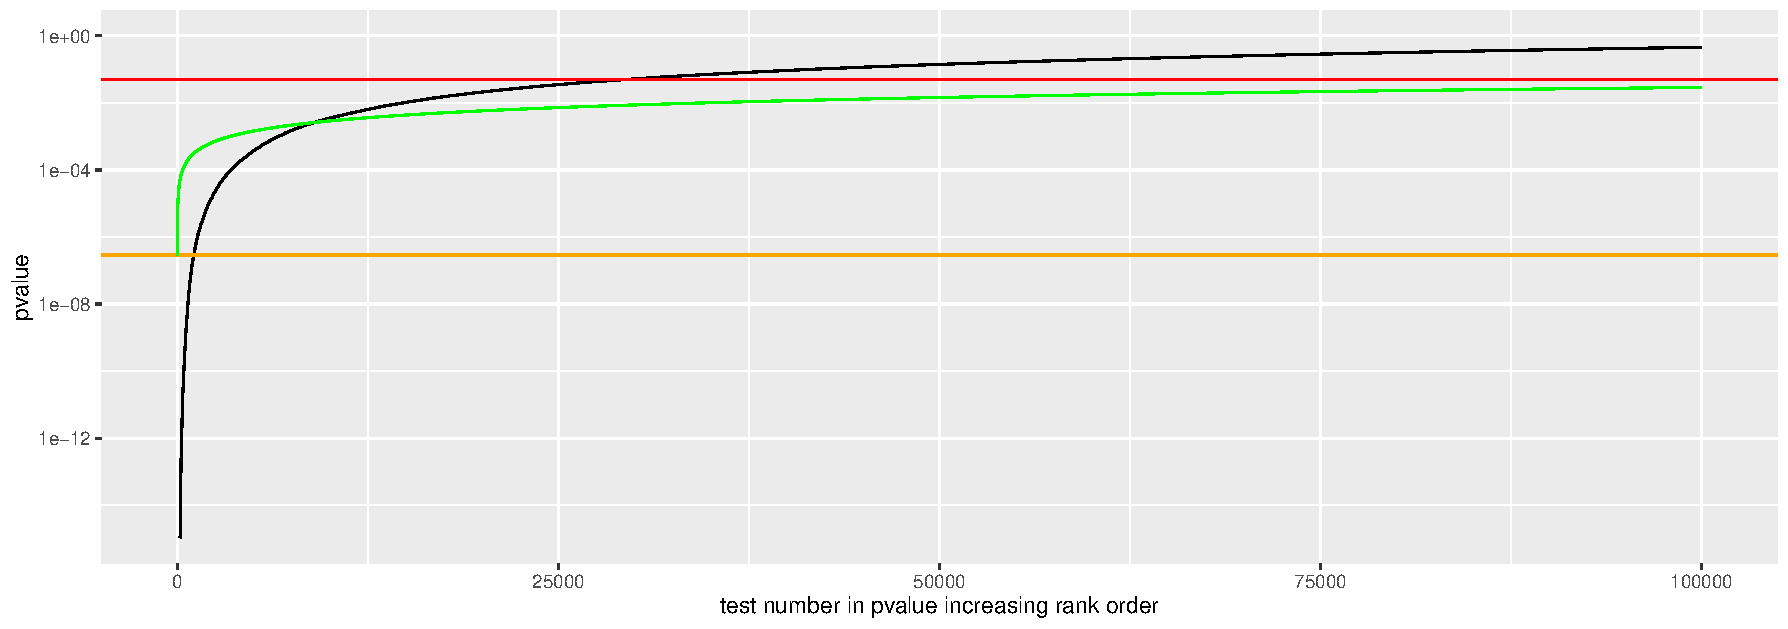
\includegraphics[width=7in]{pvals}
\end{figure}}~\spc{3}

\easysubproblem{Compute the Bonferroni threshold. Ensure that the Bonferroni is smaller than the Sidak.}\spc{4}

\easysubproblem{Compute the Sidak $\alpha$ threshold. Ensure that the Bonferroni threshold is smaller than the Sidak threshold.}\spc{4}

\easysubproblem{The Simes $\alpha$ threshold is 0.00262. Would that yield more rejections than Bonferroni? Yes / No.}\spc{-0.5}

\easysubproblem{Employing the Benjamini-Hochberg procedure, what does your number of rejections mean? Explain and be specific.}\spc{3}

\intermediatesubproblem{Why do you think the Benjamini-Hochberg procedure to control FDR has had such a huge impact on science?}\spc{10}

\easysubproblem{We looked at the illustration below during lecture, the histogram of the pvals. 

\begin{figure}[h]
\centering
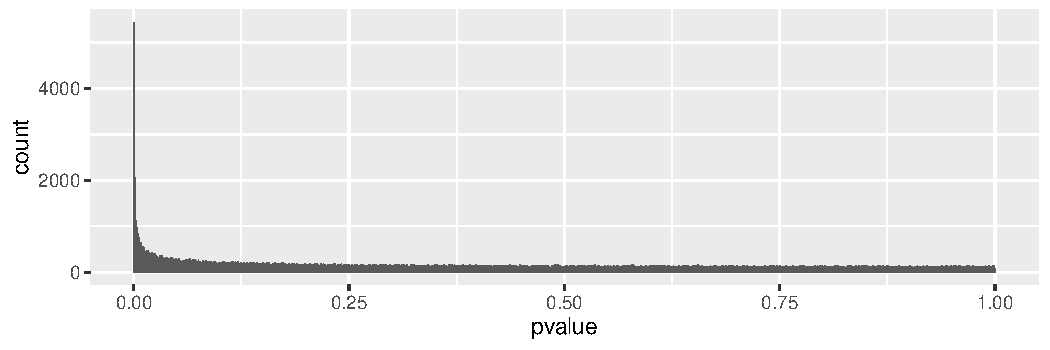
\includegraphics[width=7in]{hist_pvals}
\end{figure}

Do you believe that all $H_0$'s are true? Yes / No.}\spc{-0.5}

\hardsubproblem{Do you think that Bonferroni / Sidak / Simes are more conservative now that you've seen the plot? Explain}\spc{4}


\end{enumerate}%%%%%%%%%%%%%%%%%%%%

\problem{This is about the core thm.}

\begin{enumerate}

\easysubproblem{State the theorem's results for MLE's and MM estimators}\spc{6}

\easysubproblem{Assuming $\thetahatmle \convp \theta$ and the \qu{technical conditions} we glossed over (e.g. the MLE is not on a boundary of $\Theta$), prove that the MLE is asymptotically normal with mean $\theta$ and variance equal to the CRLB on variance.}\spc{25}

\end{enumerate}%%%%%%%%%%%%%%%%%%%%

\problem{Consider height data from 2020's MATH 369 class. We sample $n_1 = 10$ men and measured heights in inches: 67, 68, 69, 70, 70, 71, 72, 72, 73 and 73 and $n_2 = 6$ females and measured heights in inches: 59, 60, 63, 64, 64 and 64.

}

\begin{enumerate}

\easysubproblem{Over the regions of Europe, North America, Australia, and East Asia, female height is found to be normally distributed with mean 64.8in and standard deviation 2.8in (see \href{https://ourworldindata.org/human-height\#height-is-normally-distributed}{here}). We wish to test if our data deviates from this distribution. State the null and alternative hypothesis.}\spc{2}

\easysubproblem{Using these mean and standard deviation values, standardize the data for the $n_2$ female height measurements and provide the values of $z_1, ..., z_6$ below.}\spc{2}

\easysubproblem{In the following space create an illustration that plots the empirical CDF (the estimate, $\hat{F}$) of the standardized female heights. Also on this plot, graph $F_Z(z)$, the CDF of $\normnot{0}{1}$.You will have to look up the quantiles for the standard normal from Math 241. Try to make your illustration to scale as much as possible but zoom in on the y axis more than the x axis. Make the y axis as high as the space below and have y range from 0 to 1.}\spc{8}

\easysubproblem{From your plot in (c), try to estimate $D_6$, the \qu{supremum norm difference} which is the largest absolute difference between the empirical CDF and $F_Z(z)$.}\spc{1}

\easysubproblem{In the statement $\sqrt{n}D_n \convd K$, what is the name of the distribution $K$? And who proved this result? Plot a rough sketch below of the PDF of $K$. Label the axes.}\spc{3}

\easysubproblem{Run the one-sample Kolmogorov-Smirnov (K-S) test for the $H_a$ in (a) using the test statistic in (d) at $\alpha = 5\%$. Note that $F_K(1.359) = 95\%$. What is your decision?}\spc{1}


\easysubproblem{We now wish to test if the DGP's for male and female height are different. State the null and alternative hypothesis.}\spc{1}

\intermediatesubproblem{In the following space create an illustration that plots the empirical CDF of the raw female heights (not standardized). Also on this illustration, plot the empirical CDF of the raw male heights (not standardized). Try to make your illustration to scale as much as possible but zoom in on the y axis more than the x axis. Make the y axis as high as the space below and have y range from 0 to 1.}\spc{7}

\easysubproblem{From the plot in (g), try to estimate $D_{6,10}$, the two-sample \qu{supremum norm difference} which is the largest absolute difference between the two empirical CDFs.}\spc{-.5}

\easysubproblem{Run the two-sample K-S test for the $H_a$ in (g) using the test statistic in (i) at $\alpha = 5\%$. Note that $F_K(1.359) = 95\%$. What is your decision?}\spc{2}

\intermediatesubproblem{Is the quantile in the cases in (f) and (j) accurate given our sample size? To run these two K-S tests more accurately, what can you do?}\spc{1}

\end{enumerate}
\end{document}

\easysubproblem{We now wish to run Fisher's permutation test to test $H_a$ in (g). Explain the steps of the permutation test carefully. Provide the four examples from the lecture of test statistics that can be employed.}\spc{8}


\hardsubproblem{Provide an examples of a test statistic that can be employed within the permutation test that we did not discuss in class. Explain why it would work.}\spc{2}

\easysubproblem{In this dataset, what is $B_{all}$, i.e. how many possible unique resamplings are there? Can these number of resamplings be done comfortably in a modern computer?}\spc{1}

\easysubproblem{Let's employ the ratio-of-averages test statistic (even though we used difference-of-averages in class). Under $H_0$ in (g), what do you expect the value of the ratio-of-averages to be?}\spc{1}

\hardsubproblem{Prove that the true mean over all resamplings is indeed the answer from (o).}\spc{7}


\easysubproblem{Calculate the ratio-of-averages test statistic for the original data.}\spc{1}

\easysubproblem{Do one resampling of the data manually by hand (make sure you split all $n$ into partitions of sizes $n_1$ and $n_2$). Write the resampled data below. Calculate the ratio-of-averages test statistic.}\spc{7}


\easysubproblem{Below is an histogram of all $B$ resamplings. The value of the ratio of averages in the original sample data is displayed as a green vertical line.

\begin{figure}[h]
\centering
\includegraphics[width=5in]{height_ratios}
\end{figure}

Estimate the RET at $\alpha = 5\%$. Run the test and report your decision. }\spc{1}


\intermediatesubproblem{Estimate Fisher's p-value for this test.}\spc{1}


\end{enumerate}


\end{document}

